%---------------------
% START OF PREAMBLE - do not delete!
%---------------------
\documentclass[12pt]{article}
\usepackage[pdftex]{graphicx}
\usepackage{amsmath}
\usepackage{verbatim}
\DeclareGraphicsRule{*}{mps}{*}{}

%==============================================================================
% Page layout
%==============================================================================

%------------------------------------------------------------------------------
%  Define the page dimensions.
%------------------------------------------------------------------------------
\setlength{\hoffset}{0.0in}
\setlength{\oddsidemargin}{0.0in}
\setlength{\evensidemargin}{0.0in}
\setlength{\textwidth}{6.75in}

\setlength{\voffset}{0in}
\setlength{\topmargin}{-.6in}
\setlength{\headheight}{12pt}
\setlength{\headsep}{12pt}
\setlength{\textheight}{9.5in}
\renewcommand{\baselinestretch}{1.0}
\renewcommand{\labelitemi}{-}

% writing the section number and the subsection number together
% and also the subsubsection in the form of 1.a
\renewcommand\thesubsection{\arabic{section}.\alph{subsection}}
\renewcommand\thesection{Problem \arabic{section}}
%------------------------------------------------------------------------------

%---------------------
% END OF PREAMBLE - do not delete!
%---------------------

\begin{document}

%---------------------
% make the title
%---------------------
\title{Mech 568 - Assignment 01 - Finite Difference}
\author{Masoud Akbarzadeh}
\date{\today}


\maketitle

%\newpage
%---------------------

%---------------------
% begin main text
%---------------------
\section{}\label{sec:problem-1}

\subsection{Problem Statement}\label{subsec:Problem Statement}
The 1-D wave equation for an acousting wave using the finite difference method is defined As:
\begin{equation}
    \frac{\partial^2 P}{\partial t^2} = c^2 \frac{\partial^2 P}{\partial x^2}
\end{equation}

\begin{figure}
\begin{center}
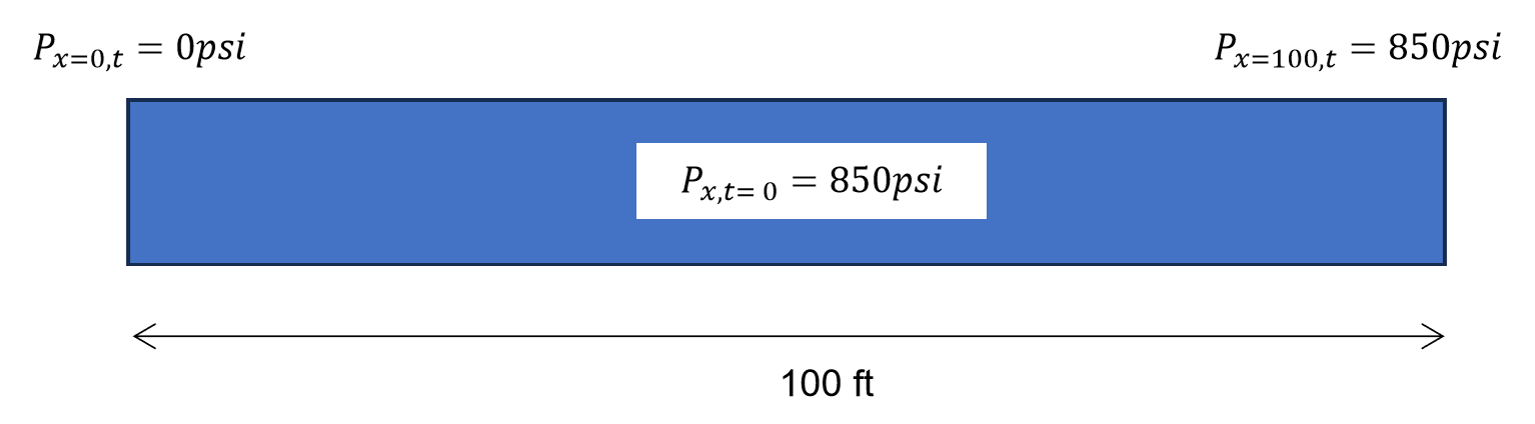
\includegraphics[width=\textwidth]{problem-statement.png}
\caption{Schematic of the boundary conditions of the 1-D pipe under an acoustic wave}{\label{fig: problem-2-c}}
\end{center}
\end{figure}

\textbf{Assumptions and conditions:}
\begin{itemize}
    \item simulating the first 0.05s of the wave with 0.001s time increments.
    \item Length of the pipe: 100 ft
    \item Number of spatial points 10 (one point each 10 ft)
    \item \( c = 1125  \frac{ft}{s} \) is the speed of sound in water.
    \item The initial pressure is the steady-state value of 850psi
    \item Since the the wave equation is a 2nd order differential with respect to time we need to initial conditions which is the pressure of 850psi at the time step 0 and -1
    \item  In order to make the equations simpler:
    \begin{equation}
    r = \frac{c^2 \Delta t^2}{\Delta x^2} 
    \end{equation}
\end{itemize}







\subsection{Explicit Method}\label{}
The equation after discretizizng the equation using the explicit method:
\begin{equation}
    P_{k+1,i} = r P_{k,i-1} + [2-2r] P_{k,i} + r P_{k,i+1} - P_{k-1,i} 
\end{equation}
Starting at the first time step at each time step, for any point this equation is solved.



\begin{figure}
\begin{center}
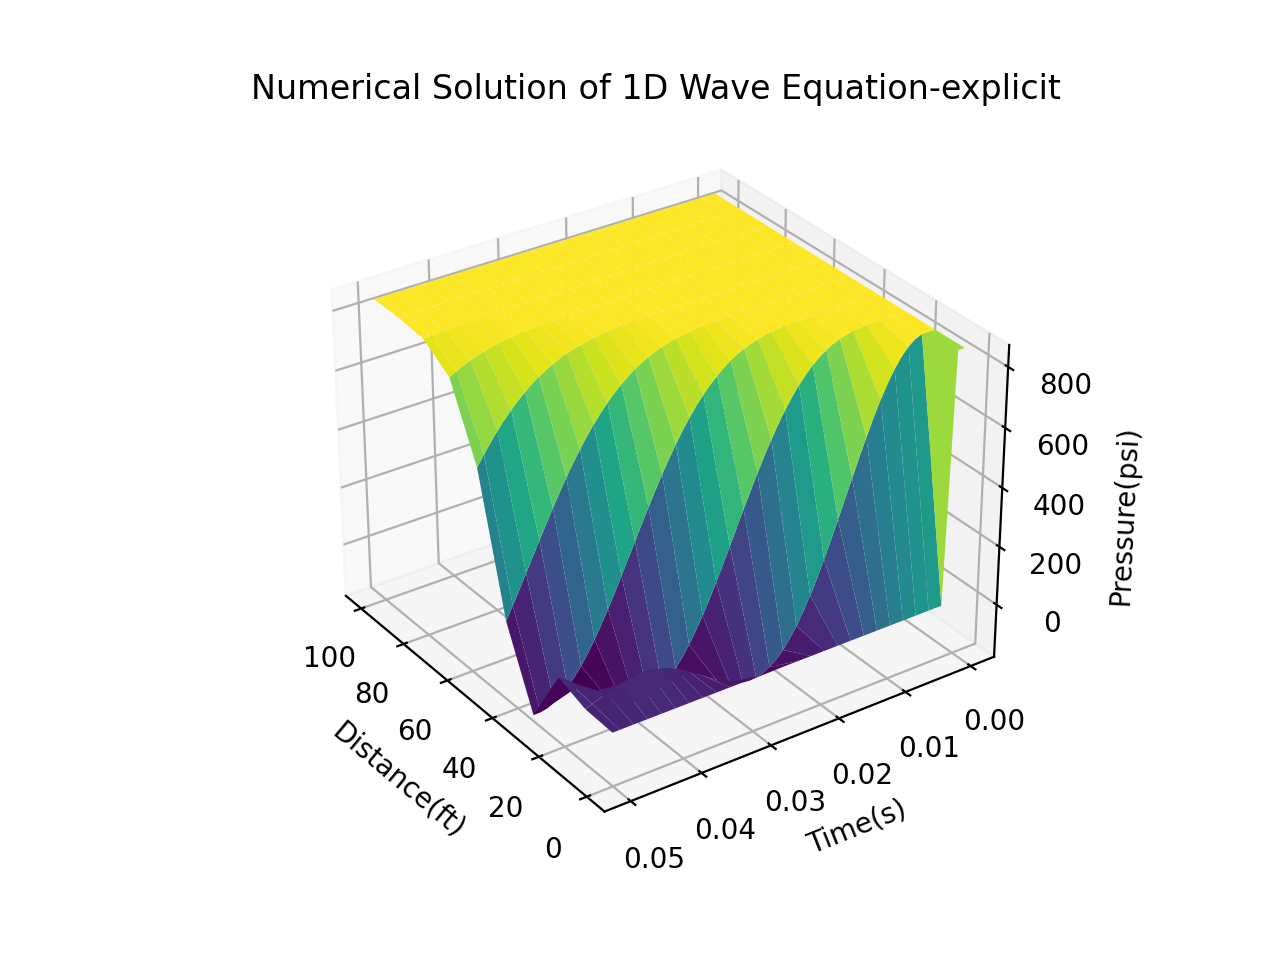
\includegraphics[width=\textwidth]{explicit_solution.png}
\caption{The plot of the solution for 1-D wave equation using explicit method}{}
\end{center}
\end{figure}

\subsection{Implicit Method}\label{}

The equation after discretizizng the equation using the Implicit method:
% \[ P_{k,i} - \frac{1}{2} P_{k-1,i} = -\frac{r}{2} P_{k+1,i-1} + \frac{(2r+1)}{2} P_{k+1,i} - \frac{r}{2} P_{k+1,i+1} \]

\begin{equation}
    P_{k,i} - \frac{1}{2} P_{k-1,i} = -\frac{r}{2} P_{k+1,i-1} + \frac{(2r+1)}{2} P_{k+1,i} - \frac{r}{2} P_{k+1,i+1}
\end{equation}

The \( P_{k,i} \) and \( P_{k-1,i} \) are know. The left side of the equation are the unknowns that make a matrix for all the points of the domain.


\begin{figure}
\begin{center}
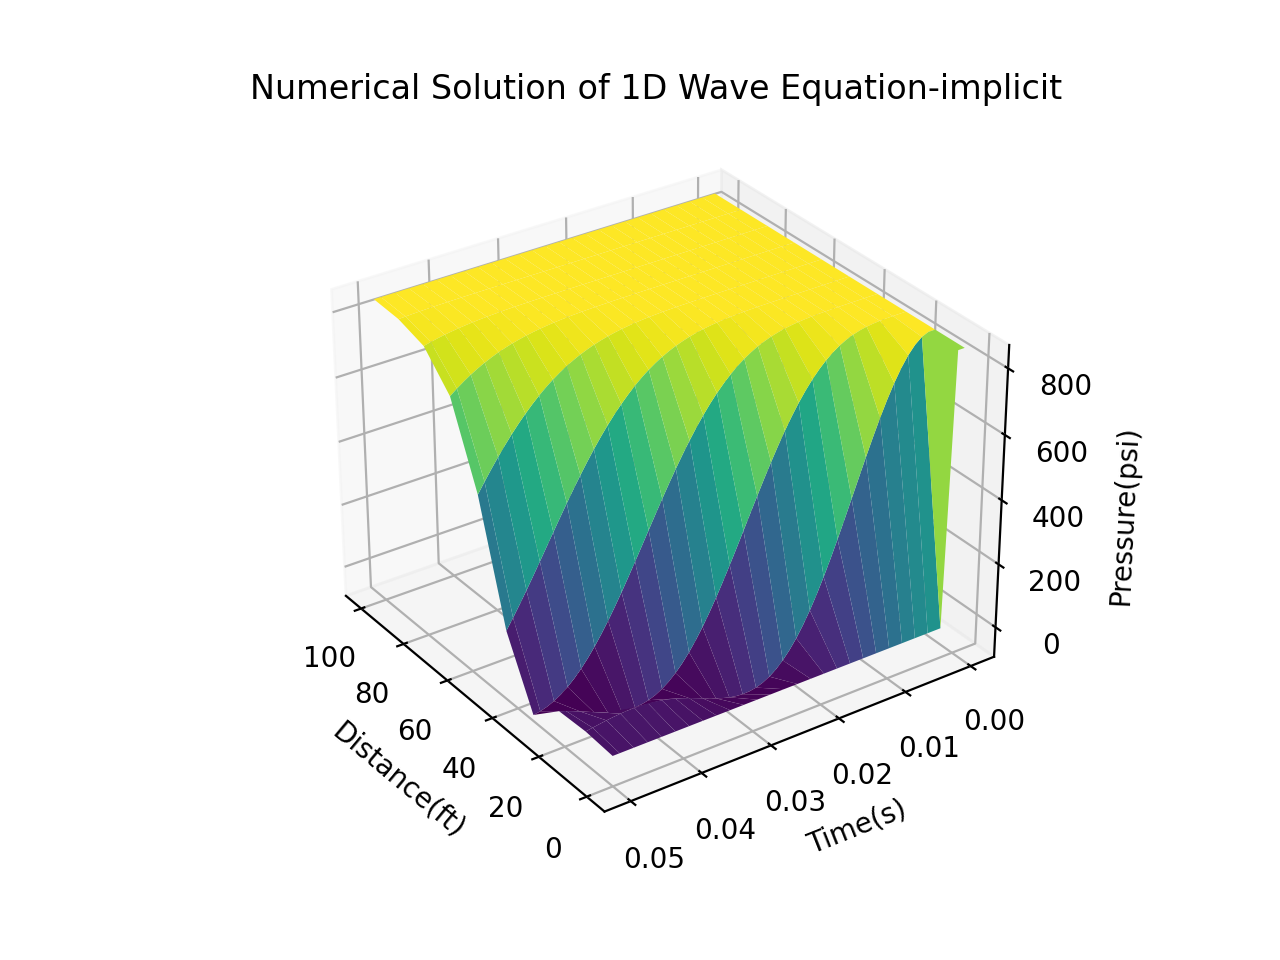
\includegraphics[width=\textwidth]{implicit_solution.png}
\caption{The plot of the solution for 1-D wave equation using implicit method}{}
\end{center}
\end{figure}
    

\subsection{Discussion}\label{}


\begin{figure}
\begin{center}
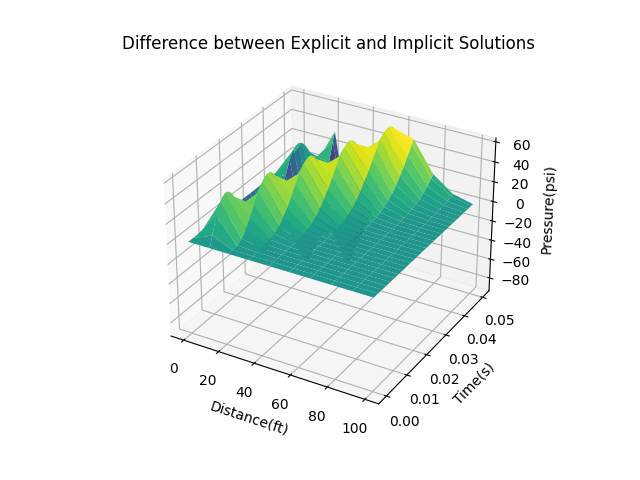
\includegraphics[width=\textwidth]{difference_solution.png}
\caption{The plot of the difference of the implicit and explicit method}{\label{fig: problem-2-c}}
\end{center}
\end{figure}



\end{document}


